\documentclass[border=10pt]{standalone}
\usepackage{tikz}\usepackage{amsmath}\usetikzlibrary{arrows.meta,decorations.markings}
\begin{document}
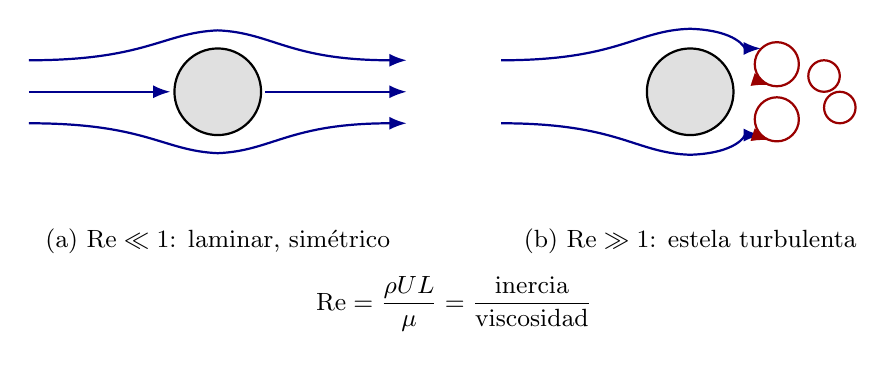
\begin{tikzpicture}[line width=0.8pt,>={Latex[length=2.2mm]}]
  % (a) bajo Re: laminar simetrico
  \fill[black!12] (0,0) circle(0.55); \draw (0,0) circle(0.55);
  \foreach \s in {1,-1}{
    \draw[blue!55!black,->] (-2.4,\s*0.4) .. controls (-0.9,\s*0.4) and (-0.7,\s*0.75) .. (0,\s*0.78) .. controls (0.7,\s*0.75) and (0.9,\s*0.4) .. (2.4,\s*0.4);}
  \draw[blue!55!black,->] (-2.4,0)--(-0.6,0); \draw[blue!55!black,->] (0.6,0)--(2.4,0);
  \node at (0,-1.9){\small (a) $\mathrm{Re}\ll1$: laminar, simétrico};
  % (b) alto Re: estela turbulenta
  \begin{scope}[xshift=6cm]
    \fill[black!12] (0,0) circle(0.55); \draw (0,0) circle(0.55);
    \foreach \s in {1,-1}{
      \draw[blue!55!black,->] (-2.4,\s*0.4) .. controls (-0.9,\s*0.4) and (-0.7,\s*0.78) .. (0,\s*0.8) .. controls (0.6,\s*0.78) and (0.7,\s*0.55) .. (0.9,\s*0.55);}
    % remolinos en la estela
    \draw[red!60!black,->,decoration={markings,mark=at position 0.7 with {\arrow{Latex}}},postaction={decorate}] (1.1,0.35) circle(0.28);
    \draw[red!60!black,<-,decoration={markings,mark=at position 0.7 with {\arrow{Latex}}},postaction={decorate}] (1.1,-0.35) circle(0.28);
    \draw[red!60!black,->] (1.7,0.2) circle(0.2); \draw[red!60!black,<-] (1.9,-0.2) circle(0.2);
    \node at (0,-1.9){\small (b) $\mathrm{Re}\gg1$: estela turbulenta};
  \end{scope}
  \node at (3,-2.7){\small $\mathrm{Re}=\dfrac{\rho U L}{\mu}=\dfrac{\text{inercia}}{\text{viscosidad}}$};
\end{tikzpicture}
\end{document}
